\documentclass[11pt, letterpaper]{article}
\usepackage[utf8]{inputenc}
\usepackage[letterpaper, margin=0.5in]{geometry}
\usepackage{amsmath}
\usepackage{amssymb}
\usepackage{amsthm}
\usepackage{graphicx}
\usepackage{listings}
\usepackage[font=scriptsize]{caption}
\usepackage{subcaption}
\usepackage{xcolor}

\definecolor{codegreen}{rgb}{0,0.6,0}
\definecolor{codegray}{rgb}{0.5,0.5,0.5}
\definecolor{codepurple}{rgb}{0.58,0,0.82}
\definecolor{backcolour}{rgb}{0.95,0.95,0.92}

\lstdefinestyle{mystyle}{
    backgroundcolor=\color{backcolour},   
    commentstyle=\color{codegreen},
    keywordstyle=\color{magenta},
    numberstyle=\tiny\color{codegray},
    stringstyle=\color{codepurple},
    basicstyle=\ttfamily\footnotesize,
    breakatwhitespace=false,         
    breaklines=true,                 
    captionpos=b,                    
    keepspaces=true,                 
    numbers=left,                    
    numbersep=5pt,                  
    showspaces=false,                
    showstringspaces=false,
    showtabs=false,                  
    tabsize=2
}

\lstset{style=mystyle}
\graphicspath{ {.} }
\captionsetup{justification=raggedright, singlelinecheck=false}

\author{Ryan Tang}
\title{STA 602 HW7}
\date{October 21st 2022}

\begin{document}
\maketitle

\section{Exercise 5.1}
We are using a the normal conjugate priors here. Hence, a Gaussian sampling model, $\theta$ is conditional normal given $\sigma^2$, and $1/\sigma^2$ follows a gamma distribution. And we want the marginal posterior for both $\theta|Y$ and $\sigma|Y$.
\begin{figure*}[!h]
  \centering
  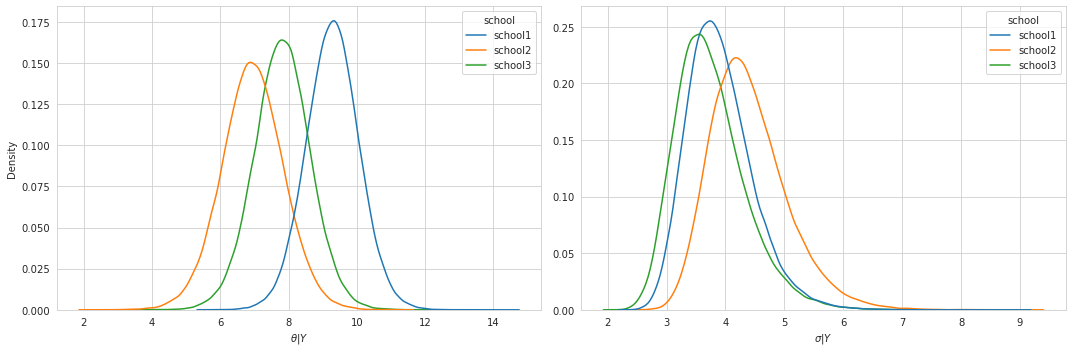
\includegraphics[width=0.9\textwidth]{5.1.a.png}
  \captionsetup{justification=centering}
  \caption{Posterior Distributions}
\end{figure*}

\paragraph{(a) Posterior Mean and Confidence Interval (CI)}
Note, according to the question, we are only showing the statistics for $\sigma|Y$, the posterior standard deviation instead of the variances.
\begin{center}
\begin{tabular}{||c c c c c||} 
 \hline
 School & $\theta|Y$ mean & $\theta|Y$ 95\% CI & $\sigma|Y$ mean & $\sigma|Y$ 95\% CI \\ [0.5ex] 
 \hline\hline
 1 & 9.29 & (7.77, 10.82) & 3.91 & (3.00, 5.18) \\ 
 \hline
 2 & 6.94 & (5.14, 8.73) & 4.39 &(3.35, 5.88) \\
 \hline
 3 & 7.81 & (6.17, 9.45) & 3.75 & (2.80, 5.13) \\
 \hline
\end{tabular}
\end{center}

\paragraph{(b) Posterior $\theta_i < \theta_j < \theta_k$ Permutations}
\begin{center}
\begin{tabular}{||c c c c||} 
 \hline
 i & j & k & Prob($\theta_i<\theta_j<\theta_k)$ \\ [0.5ex] 
 \hline\hline
 1 & 2 & 3 & 0.00572 \\ 
 \hline
 1 & 3 & 2 & 0.00368 \\
 \hline
 2 & 1 & 3 & 0.08407 \\
 \hline
 2 & 3 & 1 & 0.67347 \\
 \hline
 3 & 1 & 2 & 0.01517 \\
 \hline
 3 & 2 & 1 & 0.21789 \\
 \hline
\end{tabular}
\end{center}

\paragraph{(c) Posterior $\tilde{Y}_i < \tilde{Y}_j < \tilde{Y}_k$ Permutations}
\begin{center}
\begin{tabular}{||c c c c||} 
 \hline
 i & j & k & Prob($\tilde{Y}_i < \tilde{Y}_j < \tilde{Y}_k)$ \\ [0.5ex] 
 \hline\hline
 1 & 2 & 3 & 0.10624 \\ 
 \hline
 1 & 3 & 2 & 0.10467 \\
 \hline
 2 & 1 & 3 & 0.18327 \\
 \hline
 2 & 3 & 1 & 0.26838 \\
 \hline
 3 & 1 & 2 & 0.13745 \\
 \hline
 3 & 2 & 1 & 0.19999 \\
 \hline
\end{tabular}
\end{center}

\paragraph{(d) Posterior Probability for School 1 vs. Others}
The posterior probability that $\theta_1|Y$ is bigger than both $\theta_2|Y$ and $\theta_3|Y$ is 0.89136.
And the posterior probability that $\tilde{Y}_1|Y$ is bigger than both $\tilde{Y}_2|Y$ and $\tilde{Y}_3|Y$ is 0.46837.

\paragraph{Appendix}
The code for generating the posterior samples is included here for completeness.
\begin{lstlisting}[language=Python]
import pandas as pd
import numpy as np
import seaborn as sns
import matplotlib.pyplot as plt
import scipy.stats as stats

sns.set_style('whitegrid')

# read in the data
file_names = ["school1.dat", "school2.dat", "school3.dat"]

dfs = []
for i, fnm in enumerate(file_names):
    d = pd.read_table(fnm, header=None, names=['time'])
    d['school'] = fnm.split('.')[0]
    dfs.append(d)

df = pd.concat(dfs).reset_index(drop=True)

# priors parameters
mu0 = 5
kappa0 = 1
v0 = 2
sigma0_sq = 4

# school sufficient statistics
gp = df.groupby('school')
ns = gp.time.size()
y_bars = gp.time.mean()
vars = gp.time.var()

# posterior parameters
kns = kappa0 + ns
muns = (kappa0*mu0 + ns*y_bars) / kns
vns = v0 + ns
sigmans_sq = 1/vns * ((ns-1)*vars + v0*sigma0_sq + (kappa0*ns/kns)*(y_bars-mu0)**2)


np.random.seed(12123)

# drawing precision samples
precision_samples = stats.gamma(a=vns/2, scale=2/(vns*sigmans_sq)).rvs(size=(100000, 3))
vars_samples = 1 / precision_samples

# drawing mu samples given the precision samples
theta_samples = stats.norm(loc=muns, scale=np.sqrt(vars_samples/kns.values)).rvs()
\end{lstlisting}


\section{Exercise 5.2}



\section{Exercise 6.1}


\end{document}